\documentclass[12pt, a4paper, oneside]{ctexart}
\usepackage{amsmath, amsthm, amssymb, appendix, bm, graphicx, hyperref, mathrsfs, subfigure, parskip}
\usepackage{geometry}
\usepackage{listings, matlab-prettifier}

\geometry{left=1.5cm,right=1.5cm,top=3cm,bottom=3cm}
\linespread{1.5}
\newtheorem{theorem}{定理}[section]
\newtheorem{definition}[theorem]{定义}
\newtheorem{lemma}[theorem]{引理}
\newtheorem{corollary}[theorem]{推论}
\newtheorem{example}[theorem]{例}
\newtheorem{proposition}[theorem]{命题}
\renewcommand{\abstractname}{\Large\textbf{摘要}}
\hypersetup{hidelinks}
\setlength{\parindent}{2em}

\lstset{
	style=Matlab-editor,
	basicstyle          =   \ttfamily,          % 基本代码风格
	keywordstyle        =   \bfseries,          % 关键字风格
	commentstyle        =   \rmfamily\itshape,  % 注释的风格,斜体
	stringstyle         =   \ttfamily,  % 字符串风格
	flexiblecolumns,                % 别问为什么,加上这个
	numbers             =   left,   % 行号的位置在左边
	showspaces          =   false,  % 是否显示空格,显示了有点乱,所以不现实了
	numberstyle         =   \ttfamily,    % 行号的样式,小五号,tt等宽字体
	showstringspaces    =   false,
	captionpos          =   t,      % 这段代码的名字所呈现的位置,t指的是top上面
	frame               =   lrtb,   % 显示边框
}


\begin{document}
	
	\thispagestyle{empty}
	
	\begin{figure}
		\centering
		
\includegraphics[width = 0.9\textwidth]{logo}
	\end{figure}
	\vspace*{\fill}
	\begin{center}
		\Huge\textbf{随机音乐实验报告}
	\end{center}
	\vspace*{\fill}
	
	\begin{table}[b]
		\centering
		\large
		\begin{tabular}{ll}
			\textbf{课程:} & 音乐与数学 \\
			\textbf{组号:} & 4-14\\
			\textbf{时间:} & \today\\
		\end{tabular}
	\end{table}
	
	
	\newpage
	\pagenumbering{Roman}
	\setcounter{page}{1}
	\tableofcontents
	\newpage
	\setcounter{page}{1}
	\pagenumbering{arabic}
	
	\section{研究目的}
	统计歌曲中的“音级+时值”转移概率矩阵,通过马尔科夫链的方法产生随机音乐。
	探究产生的随机音乐与转移概率矩阵的相关性。尝试探讨生成的音乐是否好听以及可能的什么因素造成了生成的音乐好听与否。
	
	\section{理论分析}
	\subsection{马尔科夫链}
	\textbf{定义:}\quad 考虑一个随即变量的序列$X=\{X_0,X_1,\cdots,X_t,\cdots \}$,
	这里$X_t$表示时刻$t$的随机变量,$t=0,1,2,\cdots$。每个随机变量$X_t(t=0,1,2\cdots)$
	的取值集合相同,称为状态空间,表示为$S$。随机变量可以是离散的,也可以是连续的。
	以上随机变量的序列构成随机过程。\par 
	假设在时刻0的随机变量$X_0$遵循概率分布$P(X_0)=\pi_0$,称为初始状态分布。在
	某个时刻$t\geq 1$的随机变量$X_t$与前一个时刻的随机变量$X_{t-1}$之间有条件
	分布$P(X_t|X_{t-1})$,如果$X_t$只依赖于$X_{t-1}$,而不依赖于过去的随机变量
	$\{X_0,X_1,\cdots,X_{t-2}\}$,这一性质称为\textbf{马尔科夫性},即
	$$P(X_t|X_0,X_1,\cdots,X_{t-1})=P(X_t|X_{t-1}),\quad t=1,2,\cdots $$
	具有马尔科夫性的随机序列$X=\{X_0,X_1,\cdots,X_t,\cdots \}$称为\textbf{马尔科夫链},或
	马尔可夫过程。条件概率分布$P(X_t|X_{t-1})$称为马尔可夫链的转移概率分布。
	转移概率分布决定了马尔科夫链的特性。\par 
	\vspace*{1em}
	以上随机变量$X_t$只依赖于随机变量$X_{t-1}$,我们称之为一阶马尔科夫性,产生的序列
	也被称为一阶马尔可夫链。定义可扩展为n阶马尔科夫链,满足n阶马尔科夫性:
	$$P(X_t|X_0,X_1,\cdots ,X_{t-1})=P(X_t|X_{t-n},\cdots ,X_{t-2},X_{t-1})$$
	即随机变量$X_t$同时依赖于前面n个变量$X_{t-n},\cdots,X_{t-2},X_{t-1}$,而
	与之前的$X_0,X_1,\cdots$,\\$X_{t-n-1}$无关。对于本实验,只涉及一阶马尔科夫链,以下
	的“马尔科夫链”均指“一阶马尔科夫链”。
	
	\subsection{转移概率矩阵}
	若马尔科夫链在时刻$t-1$处于状态$j$,在时刻$t$移动到状态$i$,将\textbf{转移概率}记作:
	$$p_{ij}=P(X_t=i|X_{t-1}=j),\quad i,j=1,2,\cdots ,n$$
	$p_{ij}$自然满足:$$p_{ij}\geq 0,\quad \sum_{i} p_{ij}=1 $$
	如果马尔科夫链是\textbf{时间齐次的},即转移概率分布$P(X_t|X_{t-1})$与$t$无关(或
	者说$p_{ij}$与$t$无关),那么可以确定该马尔科夫链的转移概率矩阵:
	$$ P = \begin{pmatrix}
		p_{11} & p_{12} & p_{13} & \cdots \\
		p_{21} & p_{22} & p_{23} & \cdots \\
		p_{31 }& p_{32} & p_{33} & \cdots \\
		\cdots&\cdots&\cdots&\cdots
	\end{pmatrix}_{n\times n} $$\par
	
	\subsection{状态分布}
	考察马尔科夫链$X=\{X_0,X_1,\cdots,X_t,\cdots \}$在时刻
	$(t=0,1,2,\cdots)$的概率分布,称为时刻$t$的\textbf{状态分布}或\textbf{状态向量},记作:
	$$ \pi(t)= \begin{pmatrix}
		\pi_1(t)\\\pi_2(t)\\\vdots
	\end{pmatrix} ,\quad \pi_i(t)=P(X_t=i),i=1,2,\cdots $$
	马尔科夫链$X$在时刻$t$的状态分布可以由$t-1$的状态分布以及转移概率分布决定:
	$$\pi(t)=P\pi(t-1)$$
	递推可得:
	$$\pi(t)=P^t\pi(0)$$
	这里的$P^t$称为\textbf{$t$步转移概率矩阵},
	$$P^t_{ij}=P(X_t=i|X_0=j)$$
	上式说明,\textbf{马尔科夫链的状态分布由初始分布和转移概率分布(转移概率矩阵)决定}。\par 
	\vspace*{1em}
	\textbf{平稳分布:}设马尔科夫链$X=\{X_0,X_1,\cdots,X_t,\cdots \}$,其状态空间为$S$,转移概率
	矩阵为$P=(p_{ij})$,如果存在状态空间$S$上的一个分布:
	$$\pi= \begin{pmatrix}
		\pi_1\\\pi_2\\\vdots
	\end{pmatrix}$$
	使得:
	$$\pi = P\pi$$
	则称$\pi$为马尔科夫链$X=\{X_0,X_1,\cdots,X_t,\cdots \}$的平稳分布。\par 
	直观上讲,平稳分布是式$\pi(t)=P^t\pi(0)$中,令$t\rightarrow \infty$的结果。
	需要指出的是,平稳分布是否存在,即序列$\{\pi(t)\}(\pi(t)=P^t\pi(0))$是否收敛,
	与具体的转移概率分布$P$有关。对于本实验,为防止可能出现的平稳分布(这样会导致生成的音乐
	的后半部分丧失“随机性”),我们会限制$t$的最大值,不断更新$\pi(0)$获得一系列音乐片段并将它们进行拼接。
	
	\section{程序的实现}
	
	\subsection{统计歌曲}
	\subsubsection{统计策略}
	我们的统计完成了对于歌曲中主旋律的二阶马尔科夫链的统计,这样可以由代码选取使用一阶或者二阶马尔科夫链。在音高上,我们使用的统计方案是对全键盘的音单独统计而不是映射成一个统一的八度(当然因此会得到一个相对稀疏的转移矩阵),但是这样保存了非常多的信息量,以使得在实验过程中有足够的自由度,同时,我们给休止符号设定了一个特征音高,将休止也加入了统计。在其它信息方面,我们统计了每个音的时值,时值的统计也是为了给程序处理增加自由度。综上,我们的统计策略是得到一个以时值和音高的不同为标准分离的所有元素之间的转移矩阵,这将是一个较为庞大且稀疏的矩阵。
	
	\subsubsection{统计数据结构}
	\begin{enumerate}
		\item 音高:
		
		首先我们找出歌曲中的主音,此后的音高均由和主音相差的半音个数来作表达其它的各个音,然后我们会将所有的出现相对音高存在一个数组中,这个数组称为scale
		\item 时值:
		
		此后我们再次建立一个数组称为notes,这个数组的每个元素是一个二元数组,这个二元数组的第一个数标识了一个时值的相对值(例如以八分音符为基准那么十六分音符就是0.5,四分音符就是2),二元数组的第二个数标识了这个音音高在scale数组中的位置的下标(实际上会相差1,这里以下标1标识第一个元素)。那么,通过两个查询列表scale和notes我们就确定了歌曲主旋律中全部出现过的音(包含了时值和音高信息)
		\item 转移矩阵:
		
		接下来我们统计一个转移矩阵,以一阶为例,由上文我们知道,每一个时值和音高对应的那个音已经在notes数组中被分配了一个唯一下标,我们假定为notes数组的长度为N,那么我们需要一个$N\times N$的矩阵来标识任意两个下标对应的音之间是否存在关联,那么我们就将有关联的两个音之间的矩阵元记为1,其余的记为0,这样就给出了转移矩阵。
	\end{enumerate}
	
	\subsubsection{一个例子}
	比如从$C_4$到$C_5$的一个$C$大调音阶,全都为八分音符,同时我们规定八分音符为一拍,以$C_4$为主音,那么scale数组为:
	$$scale = [0, 2, 4, 5, 7, 9, 11, 12]$$
	
	notes数组为:
	$$notes = [[1,1], [1,2], [1,3], [1,4], [1,5],[1,6],[1,7],[1,8]]$$
	
	转移矩阵为$A$:
	$$matrix = A, A_{ij} = \delta_{i+1, j}$$
	
	即
	$$matrix = \begin{bmatrix}
		0 & 1 & \cdots & 0\\
		\vdots &\ddots &\ddots &\vdots\\
		0& \cdots & 1 &0
	\end{bmatrix}_{8\times 8}$$
    
    \subsection{生成随机音乐}
    \subsubsection{生成策略}
    为了避免稀疏矩阵造成的生成结果和原来的曲子太像的问题,生成时的策略采用一组一组的生成方式,具体为每两小节生成一次,每次的生成采用矩阵乘法,第一个小节从主音开始,每次左乘转移矩阵得到下一个音的概率密度,并根据概率密度随机抽取下一个音的实际结果。在整体的乐段生成上,设定乐段的最小长度以及最大长度,当乐段长度达到最小长度时开始判断是否回到主音,若回到主音则直接结束,若没有回到主音则继续生成,直到回到主音或达到乐段最长长度。
    \subsubsection{避免和原曲过于相似的方法}
    程序中采用的避免和原曲过于相似的方法是不每次更新概率向量,即某时刻的概率向量为$p_n$的情况下,若直接在此概率向量中选择一个音且使用这个音作为生成下一个音的初始状态则是常规的马尔科夫链做法,这会导致在稀疏矩阵的情况下生成的音乐和原来的统计曲子较为相似,因此这里改变了操作顺序,生成了每一个音的概率向量后,例如对于$p_n$,左乘矩阵后结果为$p_{n+1} = Ap_n$是下一个概率向量,此时利用概率向量生成当前音,并不更新概率向量,即继续使用当前的概率向量$p_n$左乘转移矩阵得到下一个概率向量$p_{n+1}$,当然,作为程序实现,每次生成后需要将概率矩阵归一化。这样,生成的音乐将和原来的统计歌曲有较大的区别。当然,这也会带来一个新的问题,就是迭代较多次数后,这样的概率向量可能会趋向于一个确定值,即相当于统计出了原来的曲子中各个音出现的概率,我们也需要想办法避免这个问题。
    \subsubsection{避免收敛于概率密度}
    程序中避免收敛于概率密度的方式是每两小节重置一下概率向量,即程序中加入一个函数判断当前概率向量与上一次重置过后的时长是否达到两个小节,若达到则以当前音对应的向量重置概率向量,这样每个概率向量的迭代次数对应的时长就不会超过两个小节,可以避免多次迭代导致概率向量收敛到最后的频率统计结果。
    \subsubsection{一个例子}
    例子中我们将以$A$表示转移矩阵,以$p_n$表示概率向量,以$v_n$表示依据概率向量抽签得到的音对应的向量,那么程序的大致操作如下:
    
    初始化过程:
    $$p_0 = v_0$$
    
    迭代过程:
    $$p_{n + 1} = Ap_n$$
    
    抽签过程:
    $$v_n\text{是}p_n\text{的依概率抽签}$$
    
    判断过程:
    \begin{enumerate}
    	\item 是否和上次重置$p_n$达到两个小节
    	
    	是:更新$p_i=v_i$
    	
    	否:使用当前$p_i$继续计算
    	
    	\item 是否达到最小乐段长度
    	
    	是:进行下一个判断
    	
    	否:继续生成
    	
    	\item 是否回归主音
    	
    	是:输出乐段
    	
    	否:进入下一个判断
    	
    	\item 是否达到最大乐段长度
    	
    	是: 输出乐段
    	
    	否:继续生成
    \end{enumerate}
    
    反复进行上述操作,即可以得到生成的乐段结果。对于这个程序实现的结果,应该说它是介于完全由上一个音马尔科夫生成和完全按出现的概率随机抽样的两种随机方法之间的一个随机生成方法,同时,作为可扩展接口,我们实际在程序里保留了选择每次重置概率向量的选项。同时,应该说我们的生成程序和稀疏矩阵的统计策略是相互耦合的,若对这个程序使用非稀疏的矩阵或者对稀疏矩阵使用完全的马尔科夫生成可能都会造成一定的后果。
    
    \subsection{程序代码}
    由于统计的转移矩阵过长(因为我们统计的是不同时值不同音高的大型稀疏矩阵),提交的文件夹里我们给出了各个统计歌曲的$.json$文件,程序由三部分函数完成,分别为reader函数,main函数和printer函数,其中printer函数和reader函数用于具体函数操作,main函数用于调用。
	而具体的转移矩阵则记录在./matrix文件中的all.mat文件中。程序具体代码在附录中给出。
    
    \section{程序结果}
	所有输出文件都在./output文件夹中。
    \subsection{纯马尔科夫过程的结果}
    利用纯粹的一阶马尔科夫模型进行生成得到的乐段如文件夹中.pdf和.midi所示,命名规则为“生成所用曲目名”+(音高)(和时值)+(一阶)。
    
    就整体的生成结果而言,不同乐曲生成的结果相对是有区别的,而且这样生成的乐段听起来更像是“蕴含有”部分意义的乐段。
    
    \subsection{二阶马尔科夫结果}
    这里做了一个简化,不考虑音符时值带来的区别后,使用了二阶的转移矩阵进行生成,生成的结果如文件夹中.pdf和.midi文件所示,命名规则为“生成所用的曲目名”+(二阶)+音高
    
    就整体而言,不同乐曲试成的结果是不同的,且二阶转移矩阵得到的生成结果就音阶而言更像原曲,但是整体相似度却反而不服考虑时值的一阶结果,这就是因为相比于考虑时值的乐段,这里的不考虑时值乐段更像是音阶练习。
    
    \subsection{改变后马尔科夫的结果}
    利用上文介绍的改变马尔科夫模型生成得到的乐段如文件夹中.pdf和.midi所示,命名规则为“生成所用曲目名”+音高和时值+(改)。
    
    就整体而言由不同乐曲这样生成的乐段的区别相对变弱了,乐段听起来像乐段的感觉也变弱了,乐段在这里变得更像是音符的一种“不蕴含有什么意义”的行进。
    
    \subsection{合并转移矩阵后的结果}
    合并了转移矩阵后的马尔科夫模型生成的乐段如文件夹中的.pdf和.midi所示,命名规则为“生成所用曲目1”+“生成所用曲目2”+比例
    
    \subsection{一些讨论}
    \subsubsection{时值对生成结果的影响}
    首先时值的加入使得生成的随机音乐的丰富性得到了非常大的提升,时值的加入使得随机结果不再是单纯的音高变化,而使得随机结果更加贴近与原本对于乐曲的预期,应该说,时值的加入,给乐曲加入了一个可能丰富意蕴的自由度。
    
    \begin{figure}[htbp]
    	\centering
    	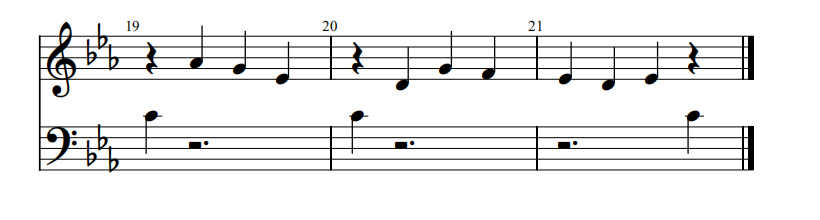
\includegraphics[width = 0.5\textwidth]{eg2}
    	\caption{不考虑时值的乐谱例子}
    \end{figure}
    
    \subsubsection{小节(轻重音)对生成结果的影响}
    实验过程中,由于我们按小节生成,并且考虑了音符的时值,因此带来了一个可能的副作用为某一个小节的开始实际上是上一小节生成的尾音的未结束部分,另考虑到休止符也被我们统计在了转移矩阵之中,实际上,某个小节的开头甚至可能是一个休止符。这会带来的问题是小节首排本该是一个重音,在随机音乐中却可能是上一个音的持续或者是休止,使得听感中预期的轻重音的节奏性质被打破,使得听感不够和谐,类似的例子如图\ref{fig:1}所示。
    
    \begin{figure}[htbp]
    	\centering
    	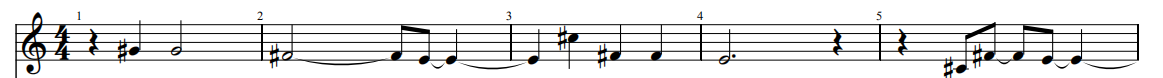
\includegraphics[width = 0.8\textwidth]{eg1}
    	\label{fig:1}
    	\caption{随机性对轻重音的影响例子}
    \end{figure}
    
    \subsubsection{重复性和随机性}
    和正常的谱写音乐相比,随机结果几乎不可能做到有一定的周期性和重复性,也不能做到比如"$ABAB$"或者"$ABAB'$"等之类的小节周期性,因此在听感而言,随机音乐的结果更像是一系列不断前进的语句,缺乏整体性的组织和架构,这就好像尝试用一些词语生成一篇文章,虽然马尔科夫链使得局域的联系得到了保留,但是以句段的长度看来,仍然无法构成一种整体性的叙述,一种有意义的表达。
    
    \subsubsection{改变马尔科夫过程造成的影响}
  	观察按小节生成的马尔科夫过程(上文介绍的我们采用的生成方式)以及传统的一阶马尔科夫过程生成的乐段,可以发现传统一阶马尔科夫过程生成的乐段听起来更像是一个传统的音乐作品,而按小节生成的马尔科夫过程形成的乐段具有更大的随机性,也因此具有更少的”特征“,更不像是一个完成的乐段而更像是一些音符的时序排列,这无疑和我们的期待是相符的。从这个角度而言,可以认为若随机抽取下一个音符是完全混沌的过程,此后若统计出了原来歌曲的各个音出现的概率,依概率抽取则相当于使用了原曲的一些信息,使得混沌的行为减弱了,进一步地,若统计了一阶马尔科夫过程,则相当于局域和原曲是相似的,这使得混沌行为进一步减弱了。而我们选用的改变的马尔科夫过程或许应该相当于介于一阶马尔科夫过程和音的概率模型之间的一种模型,因此也具有介于这两种模型之间的混沌程度。
	
	\subsubsection{二阶马尔科夫和一阶马尔科夫模型}
	考虑二阶马尔科夫模型,得到的结果就音阶演进而言相比于一阶的马尔科夫模型是更接近原曲的,这是符合预期的。实际上,做一个理想实验,倘若我们选取足够长的马尔科夫链模型,我们将可以唯一确定的生成原曲,因此,当马尔科夫模型的阶数越高时,我们往往就可以得到更为接近原曲的生成结果。但是,就实际生成的结果而言,不考虑时值的二阶马尔科夫模型和考虑时值的一阶马尔科夫模型之间的区别向我们展示了,音高和节律在乐句的进行中是同样重要的。
	
	\subsubsection{从音阶到和弦}
	当我们尝试考虑是否可能生成一个包含有和弦结构的马尔科夫模型时,我们遇到了极大的困难,即在于如何尝试平衡杂乱无章的相对音高,若和弦的几个音由不同的马尔科夫过程分别生成,则可能大量出现极度不和谐的音程,若尝试采用和弦种类的概率统计模型,从操作上看这或许是可能的,至少避免了单个和弦的不和谐,但是实际上这又会带来新的问题,即和弦和和弦之间的相对演化,若根音用马尔科夫过程生成则可能相邻和弦之间的根音音程差和和弦的几个音之间的音程差不匹配,作为结果生成的效果也不能十分令人满意。但是,值得注意的是,从生成的音阶结果来看,即使存在节奏上的变化,单个音阶的结果也往往不足够令人满意,可见历史上音乐的发展似乎确是有其道理的。
	
	\subsubsection{合并不同转移矩阵的结果}
	合并不同转移矩阵的结果如文件夹中的.pdf和.midi文件所示:但是,就结果而言,合并不同的转移矩阵后,转移矩阵被扩大了,且两首曲子的风格被中和了,实际上我们更难以分辨出这样结果和原曲的相似性。
	
	\section{总结}
	利用马尔科夫模型进行试验,似乎是给出了一个可以调节随机性程度的系统,一个演化的自由度更多的系统。尽管现代的音乐或许确实不一定需要严格满足“音乐是好听的”这一需求,但是在进行马尔科夫模拟的过程却让我们更加地认识到古典音乐在发展的过程中所加入的各种技法和操作带来的效果,或许可以作为总结的是,马尔科夫模拟的方法尽管扩大了可能的概率空间,但实际上却也同时缩小了“意义性”的空间。或许,作为玩耍,马尔科夫模型可以给出各种满足一定统计规律永无止尽的旋律片段,但是倘若从利用音乐叙述的角度而言,过大的随机性却使得“噪声”盖过了故事本身,在众多的可能性之中,我们再也没办法找到那个值得被流传的,确定的,古典的乐句。
	
	\section{小组分工}
	小组的分工如下:
	
	朱乘风、施雨希负责统计乐谱;
	
	王子谦、潘昭恺负责编写代码;
	
	李耀渝、甘景涵负责编写报告。
	
	\begin{thebibliography}{99}
		\bibitem{a}王杰. \emph{音乐与数学}[M]. 北京:北京大学出版社,2019.
	\end{thebibliography}
	
	\newpage
	
	\begin{appendices}
		\linespread{1.25}
		\renewcommand{\thesection}{\Alph{section}}
		\section{matlab运行程序}
		\subsection{代码网址}
		本项目代码使用GitHub进行维护,代码仓库位于:
		\href{https://github.com/Music-and-Math-Group-Work/Music-and-Math}{GitHub代码库}
	

		\subsection{reader函数}
		\lstinputlisting[caption={\bf reader.m}]{reader.m}
		
		\newpage
		\subsection{printer函数}
		\lstinputlisting[caption={\bf printer.m}]{printer.m}

		\newpage
		\subsection{printer函数}
		\lstinputlisting[caption={\bf merge.m}]{merge.m}
		
		\newpage
		\subsection{main函数}
		\lstinputlisting[caption={\bf main.m}]{main.m}
		 
		
	\end{appendices}
	
\end{document}
